\documentclass[12pt]{article}

 %% preamble
 \usepackage[utf8]{inputenc}
 \usepackage{amsmath}
 \usepackage[margin = 1in]{geometry}
 \usepackage{graphicx}
 \usepackage{booktabs}
 \usepackage{natbib}


 %% meta data

 \title{Demo Paper}
 \author{Olivia Dybinski\\}
 \date{September 2022}

 \begin{document}
 \maketitle

 \begin{abstract}
This is the abstract. 
 \end{abstract}


 \section{Introduction} 
 \label{sec:intro}

 Use this section to answer three questions:
 Why is the topic important/interesting?
 What has been done on this topic in the literature?
 What is your contribution?


 % roadmap
 The rest of the paper is organized as follows.
 The data will be presented in Section~2.


 \section{Data}
 \label{sec:data}

 Use this section to describe the data that helps to answer your research questions.

 \begin{figure}
    \centering
    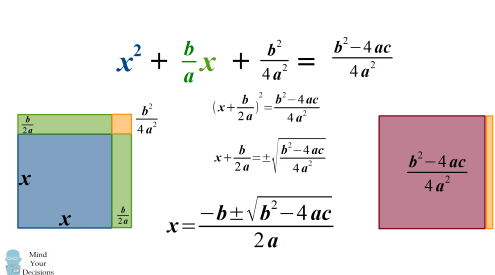
\includegraphics[width=\textwidth]{quadraticform.png}
    \caption{This is my first figure.}
    \label{fig:Quadratic Formula}
  \end{figure}

 \section{Methods}
 \label{sec:meth}

 Use this section to present the methodologies that will generate results by analyzing the data.

 A quadratic equation is an equation where the highest exponent of the given variable is 2. The standard form of a quadratic equation is $ax^2 + bx +c$ where a does not equal zero, and a, b, and c are all constants.

 The quadratic formula gives the solution to a quadratic equation in standard form, and is given by $$x=\frac{-b\pm\sqrt{b^2-4ac}}{2a}.$$

 \section{Results}
 \label{sec:results}

 \begin{table}[ht]
    \caption{This is my first table.}
    \label{tab:rv}
  \centering
  \begin{tabular}{rrr}
    \hline
  Name & Age \\ 
    \hline
    Madison & 12 \\ 
    Jacob & 4 \\ 
    Mike & 22 \\ 
    Megan & 17 \\ 
    Emily & 5 \\ 
    Jamie & 10 \\ 
     \hline
  \end{tabular}
  \end{table}

 \section{Discussion}
 \label{sec:disc}

 What are the main contributions again?

 What are the limitations of this study?

 What are worth pursuing further in the future?


 \end{document}
 

